\myframe{
  \ctr{Sumário}
}

\section*{Introdução}

\subsection*{Equações não-lineares}

\myframetop{
  \ctr{Equações não-lineares}
  \begin{equation*}
    \left\{\begin{array}{rcl}
      x_1^2 + x_2^2 & = & 4 \\
      x_1x_2 & = & 1
    \end{array}\right.
  \end{equation*}
  \begin{equation*}
    \left\{\begin{array}{rcl}
      x_1^2 + x_2^2  - e^{x_1+x_2}& = & 1 \\
      \sqrt{1 + x_1^2} + \dfrac{1}{x_2^2 + 1} & = & 1
    \end{array}\right.
  \end{equation*}
  \begin{equation*}
    \left\{\begin{array}{rcl}
      x_1x_2x_3 & = & 1 \\
      x_1x_2 + x_1x_3 + x_2x_3 & = & 3 \\
      x_1 + x_2 + x_3 & = & 3
    \end{array}\right.
  \end{equation*}
}

\myframetop{
  \ctr{Equações não-lineares}
  $$ F(x) = 0, \qquad
  F:\mathbb{R}^n\rightarrow\mathbb{R}^n. $$
  \begin{equation*}
    \left\{\begin{array}{rcl}
      x_1^2 + x_2^2 & = & 4 \\
      x_1x_2 & = & 1
    \end{array}\right.
  \end{equation*}
  $$ F(x) = \left[\begin{array}{c}
      x_1^2 + x_2^2 - 4 \\ x_1x_2 - 1
  \end{array}\right]. $$
}

\myframetop{
  \ctr{Equações não-lineares}
  \begin{equation*}
    \left\{\begin{array}{rcl}
      \color{red} x_1^2 + x_2^2
      & \color{red} =
      & \color{red} 4 \\
      \color{blue} x_1x_2
      & \color{blue} =
      & \color{blue} 1
    \end{array}\right.
  \end{equation*}
  \begin{center}
    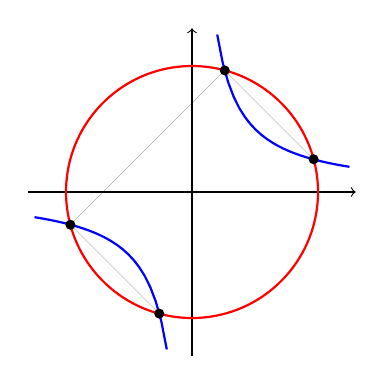
\begin{tikzpicture}[scale=0.8]
      \draw[->] (-2.6,0) -- (2.6,0);
      \draw[->] (0,-2.6) -- (0,2.6);
      \draw[red,thick] (0,0) circle (2);
      \draw[blue,thick,domain=0.4:2.5] plot (\x,{1/\x});
      \draw[blue,thick,domain=-2.5:-0.4] plot (\x,{1/\x});
      \only<2>{
        \fill (1.93,0.52) circle (0.08) --
              (0.52,1.93) circle (0.08) --
              (-1.93,-0.52) circle (0.08) --
              (-0.52,-1.93) circle (0.08);
      }
    \end{tikzpicture}
  \end{center}
}

\subsection*{A aproximação linear}

\myframetop{
  \ctr{A Aproximação linear}
  $$ F(x) \approx L(x) =  F(a) + F'(a)(x-a). $$
  $$ L(a) = F(a) \qquad L'(a) = F'(a). $$
  \begin{equation*}
    F(x) = \left[\begin{array}{c}
      x_1^2 + x_2^2 - 4 \\ x_1x_2 - 1
    \end{array}\right]
    \qquad
    F'(x) = \left[\begin{array}{cc}
      2x_1 & 2x_2 \\ x_2 & x_1
    \end{array}\right].
  \end{equation*}
  \begin{equation*}
    F(2,1) = \left[\begin{array}{c}
      1 \\ 1
    \end{array}\right]
    \qquad
    F'(2,1) = \left[\begin{array}{cc}
      4 & 2 \\ 1 & 2
    \end{array}\right].
  \end{equation*}
}

\myframe{
  \ctr{A Aproximação linear}
  \begin{equation*}
    F(2,1) = \left[\begin{array}{c}
      1 \\ 1
    \end{array}\right]
    \qquad
    F'(2,1) = \left[\begin{array}{cc}
      4 & 2 \\ 1 & 2
    \end{array}\right].
  \end{equation*}
  \begin{align*}
   L(x) & =
    \left[\begin{array}{c}
      1 \\ 1
    \end{array}\right] +
    \left[\begin{array}{cc}
      4 & 2 \\ 1 & 2
    \end{array}\right]
    \left[\begin{array}{c}
      x_1 - 2 \\ x_2 - 1
    \end{array}\right] \\
    & =
    \left[\begin{array}{c}
      4x_1 + 2x_2 - 9 \\
      x_1 + 2x_2 - 3
    \end{array}\right]
  \end{align*}
}

\myframetop{
  \ctr{Equações não-lineares}
  \begin{equation*}
    \left\{\begin{array}{rcl}
      \color{red} 4x_1 + 2x_2
      & \color{red} =
      & \color{red} 9 \\
      \color{blue} x_1 + 2x_2
      & \color{blue} =
      & \color{blue} 3
    \end{array}\right.
  \end{equation*}
  \begin{center}
    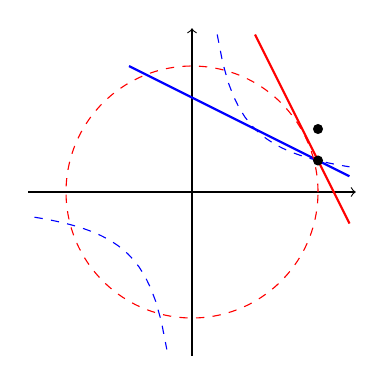
\begin{tikzpicture}[scale=0.8]
      \draw[->] (-2.6,0) -- (2.6,0);
      \draw[->] (0,-2.6) -- (0,2.6);
      \draw[red,thick,domain=1:2.5] plot (\x,{4.5 - 2*\x});
      \draw[blue,thick,domain=-1:2.5] plot (\x,{1.5 - 0.5*\x});
      \fill (2,1) circle (0.08);
      \draw[red,dashed] (0,0) circle (2);
      \draw[blue,dashed,domain=0.4:2.5] plot (\x,{1/\x});
      \draw[blue,dashed,domain=-2.5:-0.4] plot (\x,{1/\x});
      \only<2>{
        \fill (2,0.5) circle (0.08);
      }
    \end{tikzpicture}
  \end{center}
}

\subsection*{Método de Newton}

\myframe{
  \ctr{O Método de Newton}
  \begin{enumerate}
    \item Dado $x^0$, faça $k = 0$.
    \item Encontre $L_k$, a aproximação linear de $F$ em torno
      de $x^k$.
    \item Resolva o sistema linear $L_k(x) = 0$, obtendo
      $x^{k+1}$.
    \item Incremente $k$ e volte ao passo 2.
  \end{enumerate}
}

\myframe{
  \ctr{O Método de Newton}
  $$ L_k(x) = F(x^k) + F'(x^k)(x - x^k), $$
  $$ L_k(x^{k+1}) = 0, $$
  $$ x^{k+1} = x^k + d^k, $$
  $$ F(x^k) + F'(x^k)d^k = 0, $$
  $$ F'(x^k)d^k = -F(x^k). $$
}

\myframe{
  \ctr{O Método de Newton}
  \begin{enumerate}
    \item Dado $x^0$, faça $k = 0$.
    \item Encontre $d^k$, solução do sistema linear
      $F'(x^k)d^k = -F(x^k)$.
    \item Faça $x^{k+1} = x^k + d^k$.
    \item Incremente $k$ e volte ao passo 2.
  \end{enumerate}
}

\myframe{
  \ctr{O Método de Newton}
  \begin{align*}
    x^0 & = (2.00000, 1.00000), \qquad F(x^0) = (1.00000,  1.00000) \\
    x^1 & = (2.00000, 0.50000), \qquad F(x^1) = (0.25000,  0.00000) \\
    x^2 & = (1.93333, 0.51667), \qquad F(x^2) = (0.00472, -0.00111) \\
    x^3 & = (1.93185, 0.51764), \qquad F(x^3) = (0.00000, -0.00000)
  \end{align*}
  * Com 5 casas decimais
}

\section*{Otimização}

\myframe{
  \ctr{Otimização}
  $$ \min f(x), \qquad f:\mathbb{R}^n\rightarrow\mathbb{R}, f \in C^2 $$
  \begin{description}
    \item[CN1] Se $x^*$ é um minimizador local de $f$, então
      $\nabla f(x^*) = 0$.
    \item[CN2] Se $x^*$ é um minimizador local de $f$, então
      $\nabla f(x^*) = 0$ e $\nabla^2 f(x^*)$ é semidefinida positiva.
    \item[CS2] Se $\nabla f(x^*) = 0$ e $\nabla^2 f(x^*)$ é definida positiva,
      então $x^*$ é um minimizador local de $f$.
  \end{description}
}

\subsection*{O Método de Newton para otimização}

\myframe{
  \ctr{O Método de Newton para otimização}
  $$ F(x) = \nabla f(x) $$
  $$ F'(x) = \nabla^2 f(x) $$
  $$ \nabla^2 f(x^k)d^k = -\nabla f(x^k) $$
  $$ x^{k+1} = x^k + d^k $$
}

\myframetop{
  \ctr{O Método de Newton para otimização}
  \only<1>{
    $$ \nabla^2f(x^k)d + \nabla f(x^k) = 0. $$
  }
  \only<2->{
    $$ \underbrace{\nabla^2f(x^k)d + \nabla f(x^k)}_{\nabla m(d)} = 0. $$
  }
  \only<3->{
    $$ m(d) = \frac{1}{2}d^T\nabla^2 f(x^k)d + \nabla f(x^k)^Td + f(x^k).$$
  }
  \only<4->{
    $$ d^k = \arg\min_d m(d). $$
    $$ x^{k+1} = \arg\min_x m(x-x^k). $$
  }
}

\myframetop{
  \ctr{O Método de Newton para otimização}
  $$ f(x) = (1-x_1)^2 + 4(x_2 - x_1^2)^2$$
  \begin{center}
    \only<1>{ 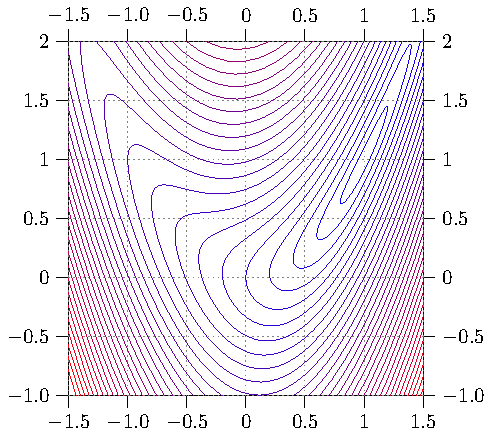
\includegraphics[height=0.6\textheight]{conicas/curvas.pdf} }

    \only<2>{ 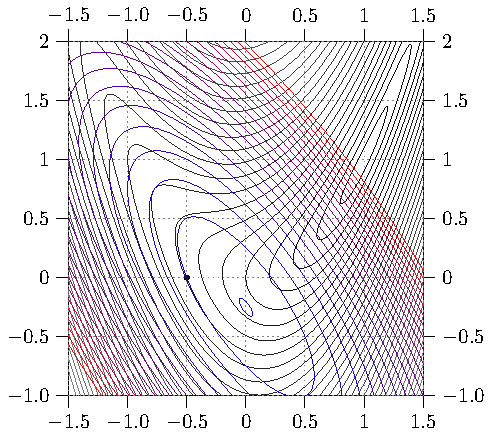
\includegraphics[height=0.6\textheight]{conicas/iter0.pdf} }

    \only<3>{ 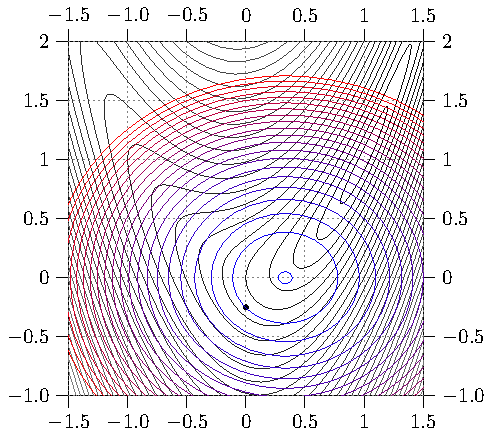
\includegraphics[height=0.6\textheight]{conicas/iter1.pdf} }

    \only<4>{ 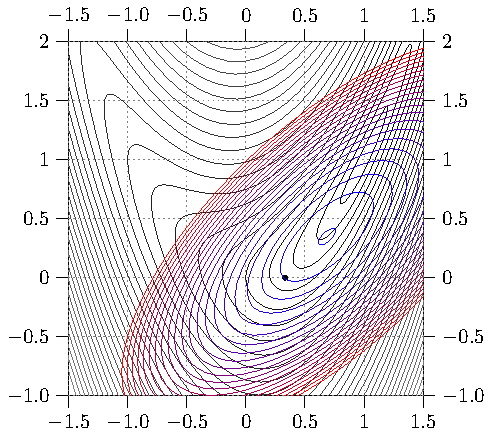
\includegraphics[height=0.6\textheight]{conicas/iter2.pdf} }

    \only<5>{ 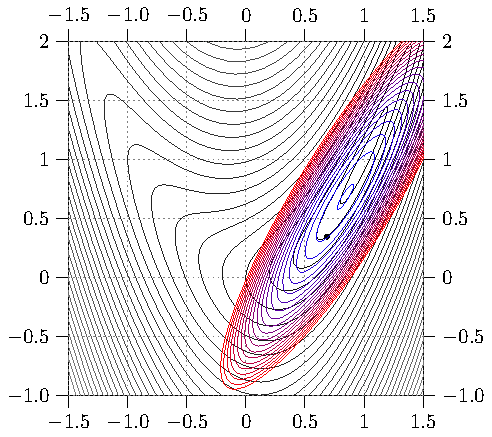
\includegraphics[height=0.6\textheight]{conicas/iter3.pdf} }

    \only<6>{ 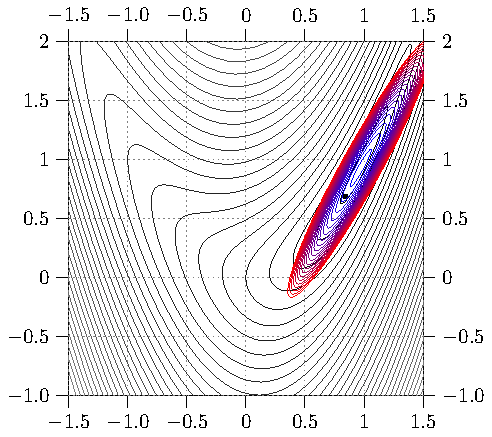
\includegraphics[height=0.6\textheight]{conicas/iter4.pdf} }

    \only<7>{ 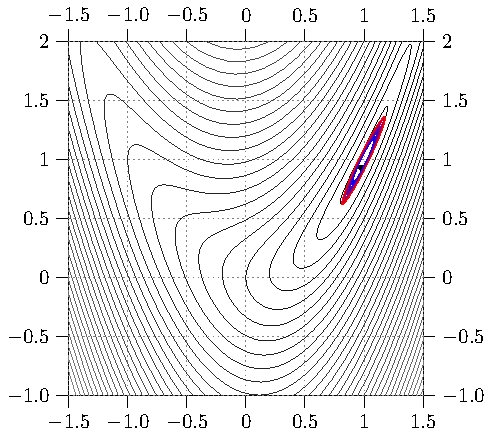
\includegraphics[height=0.6\textheight]{conicas/iter5.pdf} }
  \end{center}
}
